% 2_literature-review.tex

\cleardoublepage
\chapter{Literature review}\label{chapter:literature-review}

  \textcolor{red}{
This work aims to expand our knowledge on the operation of partially air-breathing multi-stage launch systems, by developing a trajectory for a rocket-scramjet-rocket small satellite launch system based on The University of Queensland's SPARTAN launch system. The trajectory development involves the calculation of the ascent-to-orbit of all three stages as well as the full return of the second stage, using the Pseudodospectral Method, a state of the art method of optimal control, to find the maximum payload-to-orbit trajectory profile. This optimal trajectory profile is then investigated with performance variations in the launch system, and analysed using energy methods to give insights into the trade-offs between the rocket and airbreathing stages that are unique to this type of launch system. This manner of optimal trajectory analysis allows for generalities to be made about the nature of the trajectory shape, and for understanding of the variations in the optimal trajectory with changes in the performance of the launch system to be developed.}

\textcolor{red}{
This section covers the literature available in the areas that are key to developing and analysing the trajectory for a rocket-scramjet-rocket launch system. Firstly, a background of the process of designing and flying access to space systems is given, to supply the reader with a context for the current work in the process of partially-airbreathing launch system development. 
A review of the previously developed designs of partially-airbreathing launch systems is conducted, along with an analysis of the trajectories that are able to offer valuable insights into the operations of reusable airbreathing launch systems. Of particular interest are the trajectories of partially-airbreathing launch systems that have previously been optimised to maximise a performance target, that give insights into the trajectory features that arise from the unique nature of partially-airbreathing launch systems. 
}
  
  
  
  
  \nomenclature[a]{REST}{Rectangular-to-Elliptical Shape Transition}
  
  

   
   
   
  
  \textcolor{red}{
  \section{The Launch System Design Process}
}
 \textcolor{red}{
The design of a launch system is a complex process, that involves overcoming many engineering challenges. A launch system must go through a multi-faceted design process, to take it from a definition of requirements to a physically realised and viable product. Figure \ref{fig:DesignFlow} illustrates the general design process flow for a launch system as defined by NASA\cite{Blair2001}, in which the design stages involve a repeated iterative process between the overall launch system design and compartmentalised design tasks. This compartmentalisation takes place firstly by separating the
launch system into its hardware and software subsystems, and then into general design functions that define the specifications of the subsystem design. These design functions include;
\begin{figure}[ht]
	\centering
	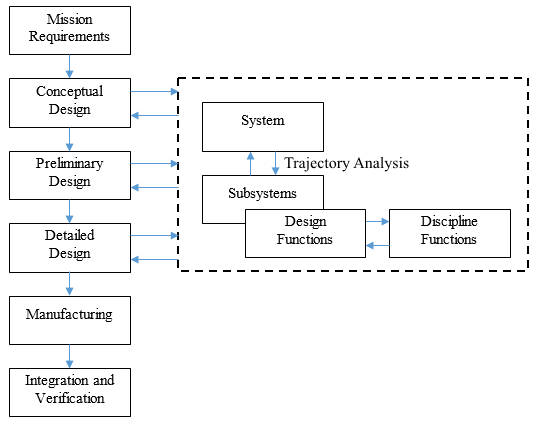
\includegraphics[width=0.7\linewidth]{figures/2_literature-review/DesignFlow}
	\caption{The general design process flow for a launch vehicle, adapted from \cite{Blair2001}}
	\label{fig:DesignFlow}
\end{figure}
\begin{itemize}
	\setlength\itemsep{.2em}
\item aerodynamics;
\item trajectory, guidance and navigation;
\item control;
\item structures;
\item thermal;
\item propulsion;
\item avionics;
\item materials;
\item and manufacturing,
\end{itemize}
among others\cite{Blair2001}. These design functions are further compartmentalised into discipline functions, which represent areas of specific speciality and expertise pertinent to the design functions. This process of compartmentalisation allows the effort associated with launch system design to be broken down into manageable amounts, and enabled the efficient utilisation of discipline and industrial specialities. 
The design process is a continuous effort to compartmentalise from the system to the subsystem, design function, and discipline function levels, and then to reintegrate and synthesise the work undertaken in order to converge on a design that is able to satisfy the overarching mission requirements\cite{Blair2001}.
} 

 \textcolor{red}{
 	Airbreathing launch systems are still in the conceptual design phase, with top level objectives and design concepts being defined. Many of the subsystems and technologies necessary to achieve airbreathing space access are in development at an academic level, and advances are necessary in multiple fields before the flight of an airbreathing launch vehicle becomes a reality. This work aims to contribute to the ongoing design of airbreathing space access vehicles by assessing the trajectory of a rocket-scramjet-rocket multi-stage launch system, contributing to the design and discipline function effort if the general mission requirement in the wider context is viewed as the development of an airbreathing space access vehicle.
 }



  \textcolor{red}{
  	\subsection{Trajectory Modelling}
  }

\textcolor{red}{XXX Citations needed}



\textcolor{red}{
	The determination and simulation of a launch system's trajectory is an integral part of the design process. The need to exit the atmosphere as efficiently as possible must be balanced against the limitations of the launch vehicle design, so that the optimal balance is found between efficiency in the design of a launch system, and the trajectory that it takes to orbit. 
	 The trajectory and design of a launch system are heavily interconnected, with the vehicle design informing the limitations and requirements imposed on the trajectory profile, and vice versa. 
	 The mass, engine performance and aerodynamic characteristics of a launch vehicle must be determined with careful consideration of the trajectory, particularly because the flight of a launch system involves vehicles flying at very high speeds and being subject to extreme aerodynamic, structural and heating loads. In the early design phases the trajectory may be very simplified, giving only a general indication of the performance of the launch system. However, even a simplified representation may be of significant use, the most relevant example of which is the Tsiolkovsky Rocket Equation, which is able to provide a first principles sizing of a rocket, assuming no external forces are acting upon it. In later design stages, more accurate trajectory models are required, including trajectories simulated to maximise the key performance metric of the launch system. These initial flight paths are then used to guide the control laws and mechanisms of the launch system.
}

\textcolor{red}{
For an airbreathing launch system, the design of a trajectory during the early design phases is particularly important. Airbreathing launch systems are typically designed using a combination of rocket and airbreathing engines, sometimes separated into multiple stages. These engines have very different requirements for operation, with rocket engines generally performing marginally better in a low density environment, at high altitudes, while airbreathing engines require relatively high density air, and require sustained atmospheric flight for operation. Figure \ref{fig:FlightCorridor} shows an example flight corridor for a partially-airbreathing launch vehicle, illustrating the upper limits of dynamic pressure at which the structural limits of the launch vehicle are met, and the lower limit of dynamic pressure at which the airbreathing engines are no longer capable of operation. 
\begin{figure}[ht]
\centering
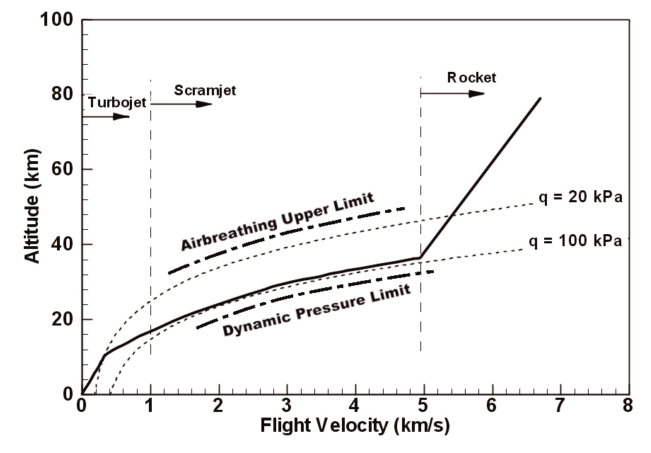
\includegraphics[width=0.7\linewidth]{figures/2_literature-review/FlightCorridor}
\caption{An example airbreathing flight corridor of a partially-airbreathing launch vehicle.}
\label{fig:FlightCorridor}
\end{figure}
This brings unique complications, as the launch system must be capable of sustained flight in-atmosphere, which results in high structural and thermal loading over long periods, that must be considered during trajectory analysis. In addition, the design trade-offs between the stages of the launch system become extremely complex, as the optimally efficient operation regime of each stage may be significantly different, resulting in the development of standard trajectories for partially-airbreathing launch vehicles being particularly challenging. 
}

\textcolor{red}{
	In addition to the complexities that arise from the addition of airbreathing engines, partially-airbreathing launch systems are also usually designed to be at least partially reusable. The return portion of the trajectory must be considered in all trajectory analysis and concurrent design for reusable launch systems. This brings additional considerations to the vehicle and trajectory design, because the vehicle must be designed to withstand the conditions of return as well as launch, and must be physically able to return and land at a suitable location. The trajectory analysis of a reusable vehicle is particularly important, as the viability of returning the vehicle to a suitable landing location must be determined, and the impact of the return trajectory on the launch flight profile must be established. 
}

  
  \section{Airbreathing Access-to-Space Systems and Their Trajectories}\label{sec:AscentTrajectories}

  \textcolor{red}{XXX I should clearly define the fidelity to which each launch is modelled.}
  \textcolor{red}{XXX Move scramjets before this, and expand this section}
  \textcolor{red}{XXX I should distinguish between launch systems using turbojets (ie virgin) and hypersonic launchers}
  \textcolor{red}{XXX I should try to keep this positive, ie. this is how the results from each study can help us}
  
    The addition of airbreathing stages to a satellite launch system to allow for partial or full reusability of a launch system has been investigated for a number of years by multiple institutions\cite{Powell1991,Wilhite1991,Varvill2008,Tsuchiya2005,Mehta2001,Preller2017b,Trefny1999,Roche2000,Young2006,Bradford2000,Gong2014}. The reduced fuel usage of airbreathing engines allows for the inclusion of systems which enable fly-back and landing of the stage in a similar manner to a conventional aircraft, potentially offering multi-launch re-use with increased launch flexibility and decreased costs\cite{Preller2017b}. However, the addition of airbreathing engines to a launch system introduces significant design challenges, and 
    no airbreathing access to space systems have yet been deployed. 
    
      \textcolor{red}{XXX more focus on design here, expand this section to discuss the details of the designs}
    The technological challenges present for an airbreathing launch system stem from the inherent limitations of jet engines. Turbojets, ramjets and scramjets all operate across different Mach number regimes, and require atmospheric flight to operate\cite{Smart2009}. 
    This means that within an airbreathing access-to-space system, a combination of various airbreathing engines and/or rockets must be used during launch.
    Figure \ref{fig:AirbreathingCorridor} shows the operating corridor for an example launch system using turbojet, scramjet, and rocket engines, indicating the point at which engine transition occurs, as well as the lower dynamic pressure limit on engine operation and the upper dynamic pressure limit on the aircraft structure.
    This operational corridor imposes unique constraints on the design of airbreathing launch systems and their trajectories. An airbreathing access to space system must be capable of resisting high structural and thermal loads, as well as being able to sustain atmospheric flight for long periods, necessitating a high lift-to-drag ratio. 
    \begin{figure}[ht]
    	\centering
    	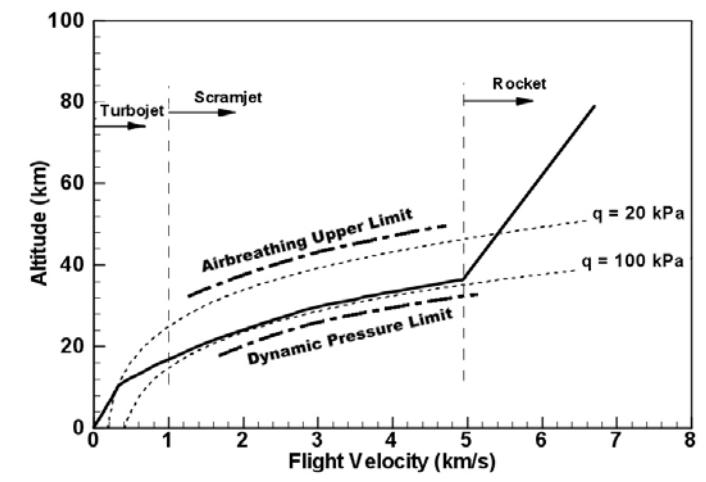
\includegraphics[width=0.7\linewidth]{AirbreathingCorridor}
    	\caption{The airbreathing vehicle flight corridor\cite{Smart2010}.}
    	\label{fig:AirbreathingCorridor}
    \end{figure}
    

    
    
Airbreathing access-to-space systems have been investigated in various forms including; single stage\cite{Powell1991,Varvill2008,Trefny1999,Roche2000,Young2006,Bradford2000}, dual stage\cite{Tsuchiya2005,Mehta2001,Gong2014,Wilhite1991} and tri stage\cite{Preller2017b} designs. 
  
  Dual stage designs have been investigated in some detail using the `spaceplane' concept by Mehta \& Bowles\cite{Mehta2001} using life cycle cost analysis in order to take flexibility and reusability into account. Mehta \& Bowles conclude that a two stage design is the optimal configuration for reusable hypersonic space access systems, however this study is only based on comparison with single stage to orbit systems, and it is more useful to consider their conclusions as an endorsement of multi stage airbreathing designs in general. They find that multi stage vehicles have higher potential for payload than single stage to orbit (SSTO) systems and have less propellant requirements, partly due to a greater atmospheric cruise capability. 
  
  
  
  
  \textcolor{red}{XXX Combine this with airbreathing access to space systems section. Make each section a more in depth review of single or multi stage launchers, and include their trajectories with them. I should strongly make the point that a well comprehensive study and optimisation of the mission of a multi stage launch system is missing. - note after, I need to think about whether it would be best to combine or keep these separate.}
  
  \textcolor{red}{I should note how much of each launch system is reusable, and also whether there is a jettisoned heat shield?}
  
  \textcolor{red}{make sure to make it clear that a three-stage / small system has not been analysed before, and that high accuracy and robust optimisation is required for a detailed trajectory analysis}
  
  \textcolor{red}{XXX Point out the propulsion systems of the different launchers, and how scramjet powered is different.}
  
  \textcolor{red}{XXX Be very specific about how they pulled up, why and to where}
  
  \textcolor{red}{XXX I should be very specific that I'm looking at a small, vertically launched, three stage system.. look at all ways that my analysis is different including whether banking during ascent is allowed (dont think banking is allowed in tsuchiya and mori during ascent) and what fidelity optimisation is used, also what engine is used (tsuchiya and mori are using a pre-cooled turbojet..)}
  
  \textcolor{red}{XXX} more papers to include:
  %https://www.jstage.jst.go.jp/article/tjsass/60/5/60_T-15-71/_pdf/-char/ja (NOTE: 2DOF)
  
  \textcolor{red}{XXX I should have a paragraph detailing why looking at variation studies is important, and compare to MDO (how it is different)}
  
  \textcolor{red}{XXX I need to look at the designs of the launch vehicles, and how they relate to their trajectories, particularly vertical vs horizontal launch}
  
  The trajectory of an airbreathing launch vehicle is more complex than that of a fully rocket-powered launch system. 
  A airbreathing launch system trajectory must be designed around a number of factors:
  \begin{itemize}
  	\item the requirement for the airbreathing stages to fly in-atmosphere,
  	\item the variable efficiency of the airbreathing engines,
  	\item the relative efficiency of the different types of engines within the system,
  	\item the aerodynamic performance of each vehicle or engine-mode of the system,
  	\item the structural limitations of the system.
  \end{itemize}
  
  A simple way to design the trajectory of an airbreathing launch system is to constrain the flight of the high speed airbreathing section to a constant dynamic pressure\cite{Olds1998,Preller2015,Punnoose2007,Kanda1996,Young2006}. 
  Constant dynamic pressure trajectories can be advantageous for an airbreathing accelerator due to the trade-off between structural loading and engine performance\cite{Olds1998}. As dynamic pressure increases so does the structural loading on the vehicle, however the performance of a ramjet or scramjet engine is directly reliant on dynamic pressure\cite{Olds1998}. A constant dynamic pressure trajectory is viewed as being an acceptable compromise between these two factors. Figure \ref{fig:constqexample} shows an example of a constant dynamic pressure trajectory flown by an airbreathing vehicle, where the airbreathing mode operates between 200-430s. 
  
  \begin{figure}[ht]
  	\centering
  	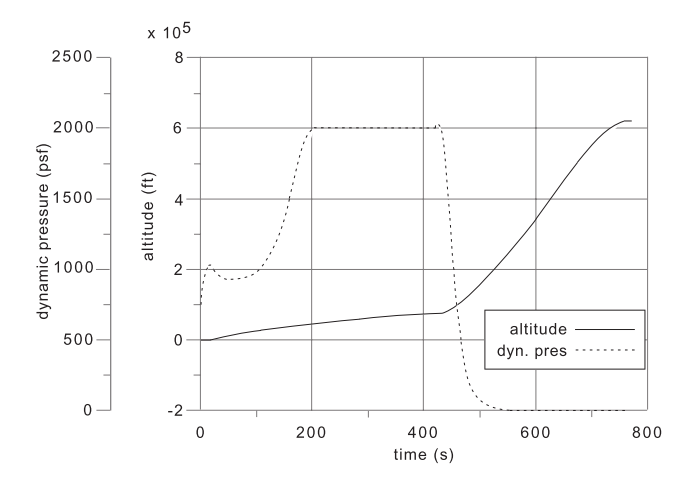
\includegraphics[width=0.9\linewidth]{ConstqExample}
  	\caption{An example of an airbreathing ascent trajectory of the Maglifter RBCC/Rocket launch vehicle\cite{Olds1998}. This trajectory shows a constant dynamic pressure section during fan-ramjet mode\cite{Olds1998}.}
  	\label{fig:constqexample}
  \end{figure}
  Although a constant dynamic pressure trajectory is likely to produce high efficiency flight for the high speed airbreathing portion of an ascent trajectory, there are a variety of factors that must be considered in designing the trajectory of a launch system. 
  For example, a constant dynamic pressure flight may produce suboptimal conditions for the switch from airbreathing engines to rocket power for exoatmospheric flight. 
  For a constant dynamic pressure trajectory the transition to rocket power will occur at a very low trajectory angle and altitude\cite{Preller2017b}. 
  It may be more optimal overall for the vehicle to fly at less than maximum dynamic pressure for a time during airbreathing engine operation, allowing the trajectory angle and altitude to be raised before the rocket engines are powered-on, increasing the efficiency of the rocket engines and reducing the dynamic pressure experienced by the rocket stage\cite{Tsuchiya2005,Wilhite1991,Mehta2001}.
  The consideration of all stages and propulsion methods, when designing the trajectory of a launch vehicle, can produce a more optimal trajectory, which maximises the performance of the launch system, eg. increasing payload-to-orbit, or increasing the range of orbits attainable by the launch vehicle.
  
  
  
  
 \textcolor{red}{XXX 
  \subsection{Single Stage Launch Systems}
}

A single stage design has the advantage of being fully contained within one vehicle, which is convenient for reusability and return trajectories. 

  	\textcolor{red}{XXX Expand this section. I should make sure to look at the type of optimisation each study uses (will note on papers in menderley).}
  	
  	\textcolor{red}{XXX I need to pull back a bit, and just discuss the trajectories in general, with less of a focus on optimisation, and more of a focus on connecting the vehicles to the trajectories. Maybe I should take all mentions of optimisation out even, and move to optimal control section?}
  	
  	\begin{figure}[h]
  		\centering
  		\begin{minipage}[b]{0.3\textwidth}
  			\centering
  			\includegraphics[width=\linewidth]{"figures/2_literature-review/Powell Vehicle"}
  			
  			\label{fig:PowellVehicle}
  		\end{minipage}	
  		\begin{minipage}[b]{0.6\textwidth}
  			\includegraphics[width=\linewidth]{"figures/2_literature-review/Powell Trajectory"}
  			
  			\label{fig:PowellTrajectory}
  		\end{minipage}
  		\caption{The single stage-to-orbit vehicle of Powell et al\cite{Powell1991} and its launch trajectory, with pull-up manoeuvre evident. $V_R$ indicates Earth relative velocity. }
  		\label{fig:Powell}
  	\end{figure}
  	Optimal trajectories have previously been developed for launch systems integrating airbreathing and rocket propulsion within single-stage-to-orbit (SSTO) vehicles\cite{Powell1991,Lu1993,Trefny1999,Roche2000,Pescetelli2012,Young2006,Bradford2000}. These optimal trajectory studies found unanimously that a pull-up manoeuvre before the end of the airbreathing engine cut-off was the optimal flight path for the SSTO airbreathing-rocket vehicles being investigated. An example of one of these vehicles, its trajectory, and associated pull-up manoeuvre is shown in Figure \ref{fig:Powell}, developed by Powell et al\cite{Powell1991}. A pull-up was found to be optimal for vehicles where the rocket engines are not ignited until circularization altitude\cite{Powell1991,Lu1993}, vehicles where the rocket engine is ignited immediately after airbreathing engine cut-off\cite{Trefny1999,Roche2000,Pescetelli2012} as well as for vehicles which operate in combined scramjet-rocket mode\cite{Young2006,Bradford2000}. For SSTO vehicles a pull-up manoeuvre is a simple trade-off between the altitude at airbreathing engine cut-off and the velocity achievable at cut-off. Due to the entire vehicle being lifted into orbit, this becomes a relatively simple problem of engine efficiency. The airbreathing engine is used for its high efficiency, until the dynamic pressure drops below the operable limit of the airbreathing engine, or until the thrust provided by the airbreathing engine is significantly counteracted by the effects of drag and gravity. 
  	
  	
  	
  	 \textcolor{red}{}
  	However, it has been suggested by Smart \& Tetlow\cite{Smart2009} that these designs suffer from severe limitations as they must contain multiple engines which add mass at later stages of the trajectory and decrease the efficiency of the vehicle. Smart \& Tetlow suggest that multistage systems offer significant improvements in payload mass fractions, and have the advantage of using airbreathing stages only within their operable range.
  	
  \textcolor{red}{XXX 
  \subsection{Two-Stage Launch Systems}
}


\textcolor{red}{XXX This is probably the key section, I need to expand on this. I should include multi stage vehicles which dont have a pull up too, and lead into how my work improves upon them.}
\textcolor{red}{XXX \cite{Kimura1999} is an example of another three stage system}

For a multi-stage to orbit vehicle, calculating the optimal trajectory for maximum payload flight is significantly more difficult. A multi-stage vehicle has one or more stage transition points, where the vehicle separates a component which is discarded or reused later, and does not continue to orbit. At a stage transition point there is a large change in the mass and aerodynamics of the launch system. 
This change in flight dynamics makes finding the optimal stage transition point more complicated. To find the optimal separation point there is a trade-off between:
\begin{itemize}
	\item the high efficiency of the scramjet engines,
	\item the thrust produced by the scramjet engines,
	\item the potential thrust of the rocket engines,
	\item the energy necessary to increase the altitude of the scramjet stage,
	\item the aerodynamic efficiency when performing the required direction change.
\end{itemize}
All of these factors must be considered in order to generate an optimal trajectory. 

\begin{figure}[!ht]
	\centering
	\begin{minipage}[b]{0.45\textwidth}
		\centering
		\includegraphics[width=\linewidth]{"figures/2_literature-review/Wilhite Booster Vehicle"}
		
		\label{fig:WilhiteVehicle}
	\end{minipage}	
	\begin{minipage}[b]{0.45\textwidth}
		\includegraphics[width=\linewidth]{"figures/2_literature-review/WilHite Booster Trajectory"}
		
		\label{fig:WilHiteTrajectory}
	\end{minipage}
	\caption{The two stage-to-orbit launch vehicle of Wilhite\cite{Wilhite1991}. The launch trajectory is shown, with pull-up indicated.}
	\label{fig:Wilhite}
\end{figure}

\begin{figure}[ht]
	\centering
	\begin{minipage}[b]{0.45\textwidth}
		\centering
		\includegraphics[width=\linewidth]{"figures/2_literature-review/Tsuchiya Vehicles"}
		
		\label{fig:TsuchiyaVehicle}
	\end{minipage}	
	\begin{minipage}[b]{0.45\textwidth}
		\includegraphics[width=\linewidth]{"figures/2_literature-review/Tsuchiya"}
		
		\label{fig:TsuchiyaTrajectory}
	\end{minipage}
	\caption{The two stage-to-orbit launch vehicle of Tsuchiya and Mori\cite{Tsuchiya2005}, with trajectories including pull-up and return for both airbreathing and airbreathing/rocket vehicles shown.}
	\label{fig:Tsuchiya}
\end{figure}

There has been a number of studies which have identified a pull-up manoeuvre as being advantageous for a multi-stage system\cite{Tsuchiya2005,Wilhite1991,Mehta2001}. However, in these studies a pull-up manoeuvre has been specified in order to decrease the dynamic pressure of the vehicle at airbreathing-rocket stage separation. 
In the studies by Tsuchiya et al.\cite{Tsuchiya2005} and Wilhite et al.\cite{Wilhite1991}, decreased dynamic pressure is necessary for the successful operation of the orbital rocket stages, of the systems under investigation. The launch vehicles and trajectories developed in these studies are shown in Figures \ref{fig:Tsuchiya} and \ref{fig:Wilhite} respectively. In these studies the airbreathing stages pull-up to the maximum allowable dynamic pressure for the rocket-powered orbital stages. When the orbital stages are able to operate, stage separation occurs. These pull-up manoeuvres demonstrate the advantages of a pull-up for the operation of the orbital stages, allowing the aerodynamic and thermal loading on the vehicle to be reduced. However, these pull-up manoeuvres are not performed as part of optimal trajectories, instead they are designed to ensure that the performance constraints of the systems are met. 
Mehta \& Bowles\cite{Mehta2001} prescribe a 2g pull-up at flight conditions of Mach 10, 95000 ft for an airbreathing stage in order to ``lower dynamic pressures and to achieve the optimal launching flight path angle for the orbiter vehicle". The launch vehicle and trajectory developed by Mehta \& Bowles is shown in Figure \ref{fig:Mehta}. This prescribed manoeuvre indicates that a pull-up before airbreathing-rocket transition is considered the optimal trajectory, however this study does not optimise the shape or magnitude of the pull-up manoeuvre, only considering the increased performance of the rocket vehicle. 

\begin{figure}[ht]
	\centering
	\begin{minipage}[b]{0.3\textwidth}
		\centering
		\includegraphics[width=\linewidth]{"figures/2_literature-review/Mehta Vehicle"}
		
		\label{fig:MehtaVehicle}
	\end{minipage}	
	\begin{minipage}[b]{0.6\textwidth}
		\includegraphics[width=\linewidth]{"figures/2_literature-review/Mehta Trajectory"}
		
		\label{fig:MehtaTrajectory}
	\end{minipage}
	\caption{The two stage-to-orbit launch system developed by Mehta and Bowles\cite{Mehta2001}, with trajectory and pull-up shown.}
	\label{fig:Mehta}
\end{figure}


  \textcolor{red}{XXX 
  \subsection{Three-Stage Launch Systems}
}
\textcolor{red}{XXX Look for other three stage designs}
	
\textcolor{red}{XXX Note here that this is a review of previous work done on the system, and that this study only uses some parts of this work. Also note limitations in previous work.}

\begin{figure}[ht]
	\centering
	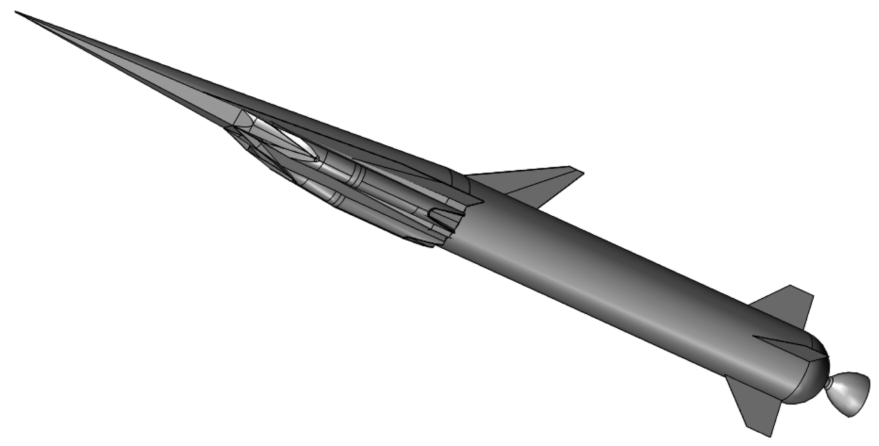
\includegraphics[width=0.7\linewidth]{SPARTAN}
	\caption{An early design of the rocket-scramjet-rocket launch system incorporating the SPARTAN\cite{Jazra2013}.}
	\label{fig:SPARTAN}
\end{figure}
The three stage, partially reusable, access to space system under development at The University of Queensland utilises the SPARTAN\cite{Jazra2013} scramjet powered vehicle as the reusable second stage, shown in Figure \ref{fig:SPARTAN}. This system is considered in this study as a representative model for three stage, airbreathing access to space system designs. This launch system is designed for small payload deliveries to orbit and will in the future utilise a fly-back rocket booster to accelerate the SPARTAN stage to minimum Mach number required for stable burn, at which point separation occurs and the second stage uses a scramjet engine to accelerate to between approximately Mach 5-9. The first and second stages are to be reusable, the first stage via conversion into a propeller powered drone, and the second stage through either a glide, or scramjet-powered flight to a suitable landing site.
The third stage will be a disposable rocket stage, which will then deliver the payload to orbit, exiting the atmosphere and performing a Hohmann transfer. 
Preliminary designs of the SPARTAN have been completed, with the shape of the SPARTAN optimised for payload delivery to heliosynchronous orbit.
Studies have indicated that the expendable third stage makes up only 8.8\% of the mass of the launch system, and that if the SPARTAN and first stage rockets are able to be reused, approximately 90\% of the launch system mass would be reusable\cite{Preller2017b}.

\begin{figure}[ht]
	\centering
	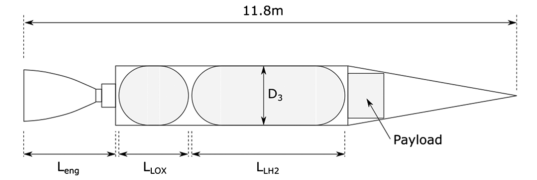
\includegraphics[width=0.7\linewidth]{figures/2_literature-review/ThirdStage}
	\caption{The third stage rocket of the rocket-scramjet-rocket launch system\cite{Preller2017b}.}
	\label{fig:ThirdStage}
\end{figure}
The third stage rocket of the rocket-scramjet-rocket launch system consists of a rocket motor, fuel tanks, structure, payload and a thermal protection system\cite{Preller2017b}, shown in Figure \ref{fig:ThirdStage}. 
The third stage rocket separates from the SPARTAN at the end of its trajectory, and performs a pull-up manoeuvre to exit the atmosphere. Once the density of the atmosphere is low enough, the thermal protection system separated from the vehicle for mass efficiency, and once exoatmospheric, the third stage performs a Hohmann transfer to reach the desired orbit. 
The third stage has to this point been designed to be powered by the Pratt \& Whitney RL-10-3A\cite{Preller2017b}, and has exhibited good performance when powered by this engine. However, the RL-10-3A is a pump-fed engine, and is likely to be prohibitively expensive for a small launch system. 
 



\begin{figure}[!ht]
	\centering
	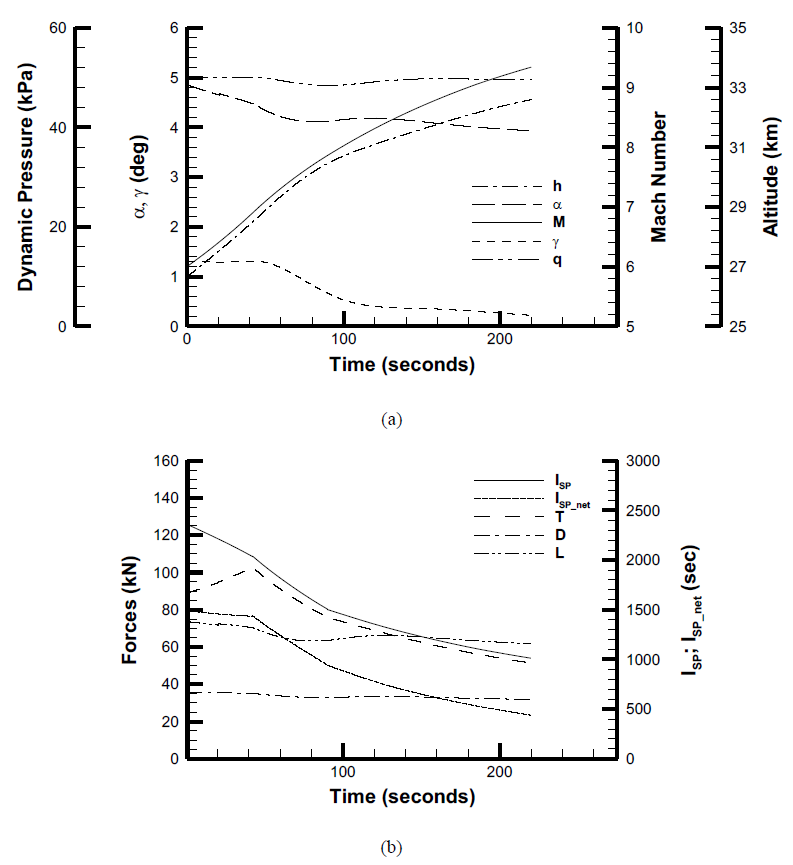
\includegraphics[width=0.9\linewidth]{figures/2_literature-review/SPARTAN_traj1}
	\caption{The flight trajectory of the SPARTAN. a) shows the physical trajectory and b) shows the forces on the vehicle and performance indicators.}
	\label{fig:SPARTAN_traj}
\end{figure}

To date, studies of the SPARTAN have assumed a constant dynamic pressure trajectory\cite{Preller2017b}.
Past studies of the SPARTAN vehicle have assumed that a fly-back to launch site is possible after third stage separation\cite{Preller2017b}. However, this fly-back has not yet been simulated. 
\begin{figure}[ht]
	\centering
	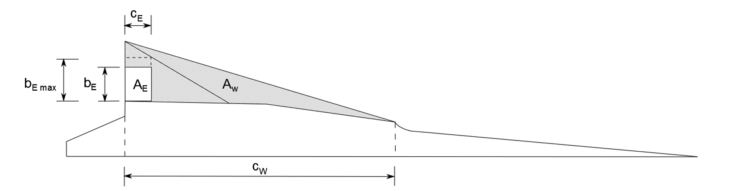
\includegraphics[width=0.7\linewidth]{figures/2_literature-review/SPARTANElevons}
	\caption{The elevons of the SPARTAN\cite{Preller2017b}.}
	\label{fig:SPARTANElevons}
\end{figure}

Figure \ref{fig:SPARTAN_traj} shows the trajectory of the SPARTAN, simulated in \textcolor{red}{three} degrees of freedom to fly close to a constant 50kPa dynamic pressure, using a pole-placement angle of attack controller\cite{Preller2017b}.
The ascent trajectory of the SPARTAN begins at Mach 6, and terminates at Mach 9.34, when the hydrogen fuel is exhausted\cite{Preller2017b}. 
The net specific impulse of the SPARTAN varies from 1492s at the beginning of the trajectory, to 439s by the time the fuel is depleted\cite{Preller2017b}. This significant decrease in efficiency means that by the end of the trajectory, the net efficiency of the SPARTAN is approximately that of a rocket\cite{Preller2017b}.

The SPARTAN is trimmed throughout the trajectory by ailerons on the wing, shown in Figure \ref{fig:SPARTANElevons}. These elevons were sized through variation of the width, $b_E$, to have an area equal to 15\% of the area of the wing, and to have a cord length, $c_E$, of 15\% of the cord length of the wing\cite{Preller2017b}. Over the flight of the SPARTAN, the flap deflection changes from 10.6$^\circ$ to 12.2$^\circ$\cite{Preller2017b}. The drag contribution of the flap varies from 14.3\% to 14.5\%, and the lift contribution from 18.8\% to 21.0\%\cite{Preller2018a}. 



This trajectory enables the delivery of 279.8kg of payload to sun synchronous orbit, when using a third stage powered by a Pratt \& Whitney RL-10-3A\cite{Preller2018a}. 
This trajectory was designed around the SPARTAN flying a constant dynamic pressure trajectory, with the third stage trajectory confirming to this constraint, and the first stage trajectory not simulated. It has been suggested that for the design of this launch system to be improved, an optimised trajectory is necessary\cite{Preller2017b}.







\section{Hypersonic Vehicle Fly-Back Trajectories}
\textcolor{red}{XXX I'm not sure how to tie this with the other sections just yet. I should maybe make the point that a skipping trajectory has not been shown to be the optimal trajectory for a hypersonic vehicle returning from launch. (It may be possible that the constraints placed on previous optimised trajectories prevented a clear skipping profile? or maybe the vehicles werent right? I should see why this is different)}

\textcolor{red}{XXX Change this to be just about non-launch vehicle trajectories, and Be clear why this section is separate. I should describe the trajectories in general in previous chapter, and then use this section to narrow down the possibilities for a system more like the SPARTAN. I should emphasize that spartan may behave more like a hypersonic glide vehicle than a reentry craft. }

\textcolor{red}{XXX I should note that the optimisation will be given the ability to perform a skipping trajectory with multiple reignitions}

\textcolor{red}{XXX I should cite Toso in this section too}

\textcolor{red}{XXX  I should have the space shuttle in thiss eciton}

The fly-back of an airbreathing launch vehicle is a crucial component of the trajectory. The ability to land a reusable launch vehicle safely in the intended location is a key requirement, and if this fly-back can transport the launch vehicle back to the initial launch location, then transport costs and turnaround times can be significantly reduced. 

There are three main methods that have been studied for potential hypersonic vehicle return; glide-back, cruise-back and boost-back. Glide-back involves the hypersonic vehicle returning to base and landing entirely using its aerodynamics. This requires sufficient lift to sustain the hypersonic vehicle over the entire return range, as well as the controllability to land the hypersonic vehicle in level flight. 
For a hypersonic trajectory a fully glide-back return flight is most likely unobtainable. This is due to the large downrange distance flown, and the large initial velocity at the beginning of the fly-back trajectory, when the vehicle is oriented away from the landing site. Multiple studies have investigated the maximum staging velocity allowable for the glide-back flight of a booster. 
In these studies, the maximum separation velocity for glide-back to be feasible has been found to be between Mach 3-4 at 30km-120km downrange distance, with higher initial velocities or longer downrange distances requiring fly-back under power\cite{Hellman,Tetlow1992}.

Cruise-back involves the inclusion of subsonic engines, which are used to power the fly-back of the hypersonic vehicle until landing similar to a conventional aircraft. These engines may be included solely for the fly-back\cite{Hellman}, or used in the acceleration phase for low velocity acceleration\cite{Mehta2001,Tetlow1992,Wilhite1991}. The addition of subsonic engines powering a constant velocity cruise-back phase allows the accelerator to return to base with a similar trajectory to that of traditional aircraft, allowing the velocity and altitude of the accelerator to be precisely controlled. However, the addition of subsonic engines necessary for cruise-back increases the mass of the vehicle significantly, leading to decreased mass efficiency and increased design complexity\cite{Hellman}. 

A preferable mode of powered fly-back is to use the existing hypersonic airbreathing engines during the return trajectory in a boost-back trajectory. Using the existing airbreathing engines allows for range to be added to a return trajectory, without the inclusion of additional engines. The hypersonic airbreathing engines can be operated at appropriate times during the fly-back, when they will be most impactful on the return trajectory range. However, the hypersonic airbreathing engines may only be used within their operating region, and vary in thrust and efficiency dependent on flight conditions. Hypersonic airbreathing engines have maximum efficiency at low Mach numbers\cite{Preller2017b}, with the thrust produced depending on the dynamic pressure and inlet conditions, which vary with the trajectory path and angle of attack of the vehicle. 

The possibility of an airbreathing vehicle reigniting high speed airbreathing engines for short periods has been investigated by Tsuchiya and Mori\cite{Tsuchiya2005}.  Tsuchiya and Mori investigate two conceptual launch vehicles; a vehicle powered solely by airbreathing propulsion returning after separation of an orbital stage at Mach 5.1, and an airbreathing/rocket vehicle returning after a separation at Mach 6.8\cite{Tsuchiya2005}.  Both vehicles use the high speed airbreathing engines during return flight. The optimal launch and return trajectories for these vehicles are shown in Figure \ref{fig:Tsuchiya}. Both vehicles ignite the airbreathing engines at around Mach 3.5 for ``several tens of seconds" to extend the range of the fly-back manoeuvres. After this, the vehicles descend and land at the launch site. 
These boosters fly to a downrange distance of 600-625km from the launch site, and less than 5\% of the vehicles initial propellant was required to return the vehicles to the initial launch sites\cite{Tsuchiya2005}.

If powered fly-back is necessary, the additional fuel weight used during this phase can negatively impact on the potential performance of a launch system. 
Optimising the fly-back trajectory of the reusable stages of a launch vehicle can decrease the amount of fuel used, and minimise the impact of the return phase. 
 The problem of optimising the fly-back of a launch vehicle for minimum fuel is analogous to maximising the range possible on a small amount of fuel, with manoeuvring. The maximum range trajectory of a hypersonic vehicle operating at high altitudes has been shown to be a `skipping' trajectory, where the altitude of the vehicle is repeatedly raised and lowered\cite{Moshman2014,Darby2011,Toso2015,Chai2015}. A skipping trajectory has been shown to be range optimal for hypersonic vehicles able to skip out of the atmosphere\cite{Eggers1957,Moshman2014}, as well as vehicles flying entirely within the atmosphere\cite{Moshman2014,Darby2011,Toso2015,Tetlow1992}. A skipping trajectory has also been shown to be optimal for an airbreathing hypersonic vehicle thrusting throughout the trajectory\cite{Kanda2007,Chai2015}. This optimised trajectory is shown in Figure \ref{fig:chai-boostskip}. The range optimal operation of the scramjet engine is shown to be repeated ignitions at the trough of each skip\cite{Chai2015}. The scramjets are ignited as the vehicle climbs after the trough, as the Mach number decreases to the minimum operable conditions of the scramjet engines\cite{Chai2015}. Minimising the Mach number during operation in this way maximises the efficiency of the scramjet engines\cite{Chai2015}.
 
 \begin{figure}[ht]
 	\centering
 	\includegraphics[width=0.9\linewidth]{"figures/2_literature-review/chai-boost skip"}
 	\caption{\textcolor{red}{An illustration of }the optimised maximum range trajectory of a hypersonic vehicle\cite{Chai2015}.}
 	\label{fig:chai-boostskip}
 \end{figure}

\textcolor{red}{
	\section{Trajectory Analysis}
}

\textcolor{red}{
	\subsection{Exergy Analysis}
}
\textcolor{red}{XXX I should maybe include some info on exergy/energy analysis in the lit review? I should be clear that the energy analysis of the trajectory is part of the significant contribution }


\section{Optimal Control}\label{sec:Optimisation}
\textcolor{red}{In Section XXX it has been established that the trajectory of a small, three stage partially-airbreathing launch system has not been defined.}

\textcolor{red}{XXX ingo: I need to clearly situate how this fits relative to GNC}

Calculating the optimal trajectory of a launch system with multiple stages and multiple modes of propulsion is a complex process. 
Defining the trajectory of a launch system purely from vehicle analysis is unlikely to yield a trajectory which maximises the performance of the system.
A simulation method is required which is able to calculate a trajectory path which maximises the performance of the launch system, while taking into account the aerodynamic and propulsive properties of each stage and propulsion mode. 
Optimal control theory is used in situations where an optimal trajectory path must be found with little prior knowledge of the shape of the trajectory. 

For an optimisation of a complex trajectory there are a variety of optimal control methods that are useful for specific problem types. These are separated into two categories: direct and indirect solution methods. Indirect methods are based on the calculus of variations or minimum principle model, and generally result in high accuracy solutions to optimisation problems\cite{Bulirsch1993}. However indirect models suffer from the drawbacks of small radii of convergence and the fact that the equations to be solved often exhibit strong nonlinearity and discontinuities. This means that indirect methods will not be solvable unless the problem is very well defined with a minimum of nonlinearity, making indirect methods unsuitable for many complex optimisation problems, such as aerospace vehicle simulations which can exhibit strong nonlinear behaviour and have a wide solution space. 

Direct methods transform an optimisation problem into a nonlinear programming (NLP) problem which can be solved computationally\cite{Stryk1992}. NLP solvers solve the optimisation problem defined as\cite{Bazaraa2013}:

\begin{equation}
Minimise \qquad f(x)
\end{equation}

\begin{equation}
Subject \quad to \qquad g_i(x)\leq0 \quad for \quad i=1,...,m
\end{equation}

\begin{equation}
and \qquad h_j(x) = 0 \quad for \quad j=1,...,n
\end{equation}

An optimisation problem that has been discretised in this form can thus be solved using any of a variety of NLP solvers. One of the most effective methods of solving twice differentiable NLP problems is sequential quadratic programming (SQP)\cite{Boggs2000} for which there is a variety of commercial solvers available such as NPSOL, SNOPT, and packages within MATLAB. 

In order for these packages to be able to solve an optimisation problem it must be presented in discretised form, and as such must be transformed using transcription techniques\cite{Kelly2015}. The task of transcribing a continuous optimisation problem into discrete NLP solvable form is not simple. SQP solvers can very easily run into convergence issues when provided with an optimisation problem which has not been well defined. Also, any transcription must be carried out with care that the accuracy of the solution is not compromised. 
There are multiple ways to approximate a continuous optimisation problem directly as an NLP problem, the most common of which are shooting and collocation methods. The choice of discretisation method can affect the stability and accuracy of the solution as well as the solution time of the problem. 

\subsection{Shooting Methods}

Shooting methods in optimal control are forward-time methods of discretisation\cite{Kelly2015}. Shooting methods explicitly enforce the dynamics of the system, and update the free conditions and system controls to move towards an optimal solution from an initial guess\cite{Kelly2015}. Shooting methods are generally simple to apply, and require little specialised knowledge to use once they have been implemented. 


\subsubsection{The Single Shooting Method}

The oldest and simplest method of approximating continuous optimisation problems as NLP problems is the direct single shooting method. Direct single shooting discretises the control function over the solution space, and solves this directly as an NLP by integrating the vehicle dynamics, or state variables, along the trajectory at each trajectory guess\cite{Betts1998,Kelly2015,Rao2009,Fasano2013}. Single shooting is simple to apply and has been used since the 1970s for rocket trajectory optimisation\cite{jezewski1971}. Single shooting methods suffer from nonlinearity problems, ie. an optimisation problem solved using the single shooting method will potentially struggle to solve if the problem exhibits even small nonlinearities, due to being unable to converge to an optimal solution. This makes the single shooting method unsuitable for complex problems such as a scramjet model, as there are many nonlinear factors inherent in atmosphere and airbreathing engine modelling.


\subsubsection{The Multiple Shooting Method}

Direct multiple shooting solves some of the instabilities of the single shooting method by splitting the trajectory into multiple shooting arcs, and collocating these at specific time points\cite{Betts1998,Kelly2015,Rao2009,Fasano2013}. This creates a system of discontinuities, illustrated in Figure \ref{fig:multipleshooting}, which are gradually minimised by the solver algorithm until the trajectory is continuous. These discontinuities allow greater flexibility for the solver than is afforded by the single shooting method. 

\begin{figure}[ht]
	\centering
	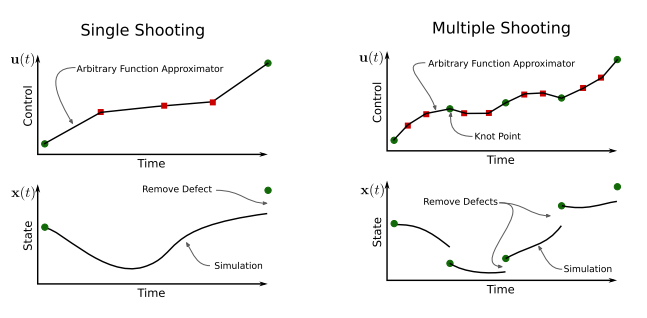
\includegraphics[width=0.9\linewidth]{SingleMultiple}
	\caption{A comparison of single shooting and multiple shooting\cite{Kelly2015}.}
	\label{fig:multipleshooting}
\end{figure}

The multiple shooting method has greatly improved convergence compared to the single shooting method, removing much of the susceptibility to instabilities resulting from nonlinear effects. However, the multiple shooting approach still suffers from a relatively small radius of convergence and slow computation times\cite{Fasano2013}. Radius of convergence is extremely important to this study as the optimal solution cannot be approximated to a great degree of accuracy, and as such multiple shooting was deemed inappropriate for this study. It was desired to find a method with a global radius of convergence to apply to the optimisation problem being considered.

\subsection{Collocation Methods}

Collocation methods are arguably the most powerful methods for solving optimal control problems\cite{Rao2009}. Collocation methods are simultaneous methods, where both the states and controls are approximated using a specific form of functional\cite{Kelly2015,Rao2009}. In these methods, the dynamics of the system are not explicitly enforced, but instead are constrained at specified points along the trajectory, called collocation points, or nodes\cite{Kelly2015}. This means that the derivative of the state functions become a constraint within the NLP, being equated to the polynomial approximation functions by the solver algorithm. 
Collocation methods provide larger radius of convergence, greater robustness, and smaller computational times compared to multiple shooting\cite{Fasano2013}. However, the solution accuracy of collocation methods is less than that of multiple shooting methods\cite{Fasano2013}, although this can be improved through the choice of basis functions used for collocation\cite{Rao2009}.

Collocation methods can be represented in two ways; \textsf{h} and \textsf{p} schemes\cite{Kelly2015}. \textsf{p} schemes, or global methods, represent the entire trajectory as high order polynomials, and converge by increasing the order of these polynomial\cite{Kelly2015}. This method works well if the underlying solution is smooth, however, if there are discontinuities present, a \textsf{p} scheme will fail\cite{Kelly2015}. \textsf{h} schemes separate the trajectory into a series of medium order polynomials, stitched together at set points using defect constraints, similarly to the multiple shooting method\cite{Kelly2015,Rao2009,Ross2004}. These joining points are called knot points\cite{Kelly2015,Ross2004}. A comparison between \textsf{h} and \textsf{p} methods is shown in Figure \ref{fig:HPExamples}.

\begin{figure}[ht]
	\centering
	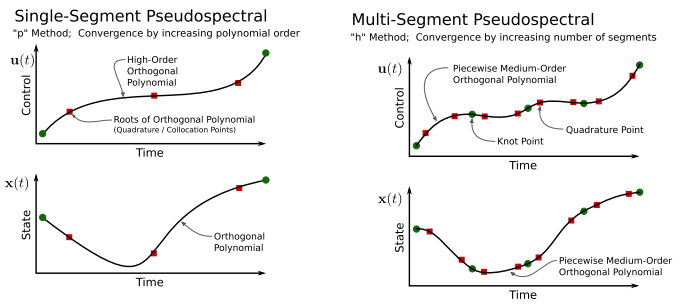
\includegraphics[width=0.9\linewidth]{figures/2_literature-review/HPExamples}
	\caption{Examples of \textsf{h} and \textsf{p} collocation methods\cite{Kelly2015}.}
	\label{fig:HPExamples}
\end{figure}

\subsubsection{The Pseudospectral Method}\label{sec:PS}


The most accurate and effective type of collocation methods use orthogonal polynomials to approximate the state and control functionals\cite{Fahroo2000}. In trajectory optimisation, this type of collocation is referred to as the pseudospectral method\cite{Kelly2015}. 
The pseudospectral method was first introduced in 1972 by Kreiss \& Oliger\cite{Kreiss1972} as an efficient way to compute meteorology and oceanography problems. The pseudospectral method has recently garnered a large amount of attention for its ability to rapidly and accurately solve a wide variety of optimal control problems.  When a solution is well behaved and smooth, the pseudospectral method converges at an exponential rate, with a high accuracy known as spectral accuracy\cite{Ross2004,Darby2011a}. 

The pseudospectral method employs the use of orthogonal polynomials such as Legendre or Chebychev polynomials to approximate the state and control functions.
This approximation is used to transcribe the optimal control problem into a nonlinear programming problem (NLP) through collocation. This process involves mapping the time domain of the system is to the time interval $[-1,+1]$, and discretising the approximated dynamics at a specific set of points, obtained from Gaussian quadrature\cite{Fahroo2000,Huntington2007,Kelly2015,Rao2009,Garg2011}. 
There are multiple types of pseudpospectral methods, distinguished by the polynomial and collocation points used. Usually, these polynomials are Chebyshev or Lagrange polynomials\cite{Fahroo2000,Rao2009}, and the collocation points are the roots of a Legendre polynomial\cite{Garg2009}. Chebyshev polynomials have been used since the introduction of pseudospectral methods in optimal control, but have been superseded in many cases by Lagrange polynomials, which offer simpler collocation conditions\cite{Rao2009}. 
There are many possible types of collocation nodes, although there are three most commonly used sets; Legendre-Gauss (LG); Legendre-Gauss-Radau (LGR); and Legendre-Gauss-Lobatto (LGL)\cite{Garg2009,Rao2009}. The choice of collocation type determines how the roots of the problem are calculated, and changes the formulation of the problem slightly\cite{Garg2009}. Practically, there is very little difference between these node sets\cite{Garg2009}.
Detailed information on the pseudospectral information may be found in Reference \cite{Huntington2007}.


The pseudospectral method is usually employed as a \textsf{p} method, where a global polynomial is used, and convergence is achieved by increasing the order of this polynomial\cite{Rao2009}. Recently, \textsf{hp}-adaptive pseudospectral methods have been introduced, which segment the mesh using an h method, whilst also having a variable polynomial degree, as in the \textsf{p} method\cite{Darby2011a}. These \textsf{hp} methods converge by varying the degree of the approximating polynomial as well as the number of segments simultaneously. Utilising both \textsf{h} and \textsf{p} methods improves the accuracy and robustness of the solution, as illustrated in Figure \ref{fig:OptimisationMethodComparisonChai}, from a study by Chai et al.\cite{Chai2015} comparing the single shooting method to \textsf{p} (Gauss) and \textsf{hp}-adaptive pseudospectral methods. Additionally, the \textsf{hp}-adaptive method decreases the computational effort and memory usage necessary during the solution process\cite{Darby2011a,Chai2015}. 


\begin{figure}[ht]
	\centering
	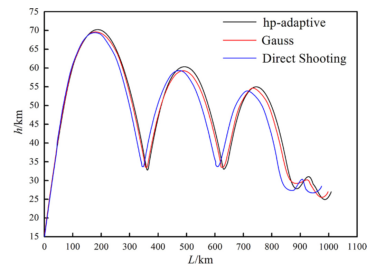
\includegraphics[width=0.7\linewidth]{figures/2_literature-review/OptimisationMethodComparisonChai}
	\caption{Comparison of optimisation techniques\cite{Chai2015}. A hypersonic vehicle is optimised for maximum range. The \textsf{hp}-adaptive method can be observed to have produced the most optimal result.}
	\label{fig:OptimisationMethodComparisonChai}
\end{figure}

A secondary usability advantage of the pseudospectral method is the ability to generate Hamiltonian and costate values easily\cite{Gong2010,Fahroo2001,Rao2009}. The Hamiltonian and costate values allow a solution to easily and quickly be checked to determine if some of the necessary conditions for optimality are being met. This is useful to determine if the optimal solution calculated by the pseudospectral solver is valid.


The pseudospectral method has been proven to be extremely effective for simulations in aerospace applications and has been proven in flight applications such as the zero propellant manoeuvre of the International Space Station in 2007, where the ISS was rotated 180 degrees without any propellant used following a pseudospectral method solution\cite{Bedrossian}. 
The pseudospectral method has been used successfully in a multitude of studies for the trajectory optimisation of hypersonic vehicles\cite{Li2012,Josselyn2002a,Zhao2013,Tian2011,Darby2011,Chai2015,Rizvi2015,Moshman2014,Yang2017,Kodera2014}. 
These results indicate that the pseudospectral method is robust for complex, nonlinear systems, and that the pseudospectral method can be used for systems with many state variables.


\section{Available Optimal Control Solvers}\label{sec:optsolvers}

There are a number of optimal control solvers available, both commercially and open source. A summary of the most prominent available solvers is shown in Table \ref{table:programs}. These programs are mostly general solvers, and must be configured specifically in order to solve a particular optimal control problem. The exception is ASTOS\cite{astos}, which is a standalone program designed for aerospace trajectory optimisation.

Functionally, most of the available solvers are similar in operation. The states and controls of the optimal control problem are defined to the program by the user, along with any constraints; continuous or endpoint. The cost function of the problem is input, and dynamic model of the system is defined. An initial guess is provided, and once activated, the solver will move toward an optimal solution from this initial guess. 
The most significant practical difference between the solvers lies in the robustness of the optimal solution, ie. how easily a particular solver is able to converge to the optimal solution. For a simple and continuous optimisation problem all solvers will be able to approach the same solution (though with varying efficiency). However, for a complex and nonlinear optimisation problem, some solvers will converge much more easily and rapidly than others. Generally, this stems from the underlying transcription method used. 
The most common form of discretisation used by these solvers is the pseudospectral method, although other forms of collocation, as well as multiple shooting, are also used. Of the methods used, \textsf{hp}-adaptive pseudospectral methods exhibit the best convergence and accuracy properties\cite{Chai2015}. The readily available packages which utilise \textsf{hp}-adaptive pseudospectral methods are GPOPS-2\cite{Rao2010} and ICLOCS2\cite{iclocs}.

ICLOCS2 is a software package in the alpha stages of development, which is based upon ICLOCS, a multiple shooting solver\cite{iclocs}. ICLOCS2 is able to implement a range of transcription methods, including a \textsf{hp}-adaptive Legendre-Gauss Pseudospectral method\cite{iclocs}. As ICLOCS2 is relatively new at the time of writing, it has not yet been implemented in any published works and documentation is limited. 

GPOPS-2 is a proprietary \textsf{hp}-adaptive pseudospectral method solver, which implements a variety of \textsf{hp}-adaptive pseudospectral methods, so that the best method may be chosen for a given problem\cite{Rao2010}. GPOPS-2 is specifically designed to be as flexible as possible, to accommodate for a wide range of problem formulations\cite{Rao2010}. GPOPS-2 is well proven in aerospace applications, and has been used for spacecraft orbit optimisation as well as in-atmosphere trajectory optimisation\cite{Rizvi2015,Lipp2014}. GPOPS-2 is well suited to solving multi-phase optimal control problems, which is necessary for efficient multi-stage launch optimisation\cite{Rao2010}. GPOPS-2 represents the state of the art in trajectory optimisation software, and as such is used by a number of institutions around the world. 

Both ICLOCS2 and GPOPS-2 uses IPOPT\cite{Wachter2006} (Interior Point OPTimizer) as the standard nonlinear programming solver (with the option of installing others). IPOPT is a widely used open source nonlinear optimisation package which utilises an interior point line search filter method. 

\begin{table}[ht]
	
	\begin{tabular}{|c|c|c| p{4cm}|}
		\hline \textbf{Software} & \textbf{Publisher} & \textbf{Platform} & \textbf{Optimisation Type} \\ 
		\hline DIDO\cite{Ross2002} & Elissar Global & MATLAB & Chebychev Pseudospectral \\ 
		\hline GPOPS II\cite{Rao2010} & RP Optimization Research & MATLAB & \textsf{hp}-Adaptive Legendre-Gauss-Radau Pseudospectral \\ 
		\hline PROPT (IPOPT)\cite{Rutquist2010}& TOMLAB & MATLAB & Legendre-Gauss  Pseudospectral  \\ 
		\hline ICLOCS2\cite{iclocs} & Imperial College & MATLAB &  Multiple Shooting / \textsf{hp}-adaptive Legendre-Gauss Pseudospectral  \\ 
		\hline POST2\cite{WilliamColson} & NASA & FORTRAN & Direct Shooting \\ 
		\hline OTIS\cite{otis} & NASA  & Fortran & Pseudospectral + Various  \\ 
		\hline TRANSWORHP\cite{Wassel2013} & ESA & Fortran/C++ & Full Discretisation \\ 
		\hline ASTOS\cite{astos} & Astos Solutions & Standalone & Multiple Shooting/Collocation  \\  
		\hline ACADO\cite{Houska2011} & Open Source & C++ &  Direct \\  
		\hline JModelica\cite{jmodelica} & Modelon AB, Open Source & Modelica/Python &  Collocation/ Pseudospectral \\  
		
		\hline 
	\end{tabular} 
	
	\caption{Summary of programs capable of pseudospectral optimisation.}
	\label{table:programs}
\end{table}




\section{Pseudospectral Method Optimisation in Aerospace Applications}
Optimal control theory has been widely used in aerospace applications, including being used to optimise the launch of airbreathing hypersonic launch vehicles\cite{Powell1991,Lu1993,Trefny1999,Roche2000,Pescetelli2012,Young2006}, \textcolor{red}{as detailed in Section \ref{sec:AscentTrajectories}}.










 





\section{Modelling and Design}



\subsection{Scramjet Engine Modelling}\label{sec:enginemodel}
\begin{figure}
	\centering
	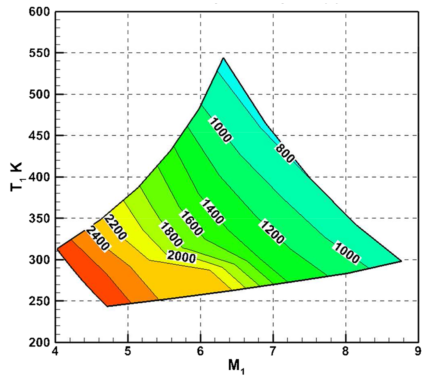
\includegraphics[width=0.7\linewidth]{figures/2_literature-review/C-REST}
	\caption{The C-RESTM10 propulsion database, specific impulse.}
	\label{fig:C-REST}
\end{figure}
To deliver a payload to orbit, the SPARTAN uses four Rectangular-to-Elliptical Shape Transition (REST) scramjet engines, with inlets configured to allow installation on a conical forebody (C-REST). The C-REST engines, which the SPARTAN uses, have been configured to fly between Mach 5 and 10. This type of engine is known as a C-RESTM10 engine\cite{Preller2017b}. The REST engine has been shown experimentally to operate successfully at off design conditions\cite{Smart2006,Smart2009a}, and has shown good agreements with numerical CFD models\cite{Smart2009a}. 

A C-RESTM10 propulsion database has been used in previous studies to model the scramjet engines of the SPARTAN\cite{Preller2017b}. The specific impulse profile of the C-RESTM10 engine, taken from the C-RESTM10 propulsion database, is shown in Figure \ref{fig:C-REST}. This database has been created through separate modelling of the compression within the inlet, combustion within the combustor, and expansion through the internal nozzle\cite{Preller2018a}. The inlet compression was modelled by performance curves based on a set of CFD solutions\cite{Preller2018a}. These performance curves were used to obtain the flow conditions at the end of the inlet. The combustor was modelled using quasi-one-dimentional cycle analysis, assuming a combustion efficiency of 80\%\cite{Preller2018a}. Lastly, the properties at the end of the combustor were expanded assuming a nozzle efficiency of 90\%\cite{Preller2018a}.
The C-RESTM10 is designed for operation at M$_0$ = 10, and the contraction ratio and combustor divergence are not optimal for operation at low Mach numbers. At low Mach numbers, an equivalence ratio of 1 may cause the flow to choke and unstart. 
Consequently, an equivalence ratio of less than 1 was set at low Mach numbers, in order to avoid unstart\cite{Preller2018a}. At these Mach numbers, the C-REST engines are operating in dual-mode\cite{Preller2018a}. 





\subsection{Aerodynamic Analysis}


Simulating the trajectory of access to space systems requires the aerodynamics of each stage of the launch system to be characterised at every flight condition experienced during launch. For this to be possible, it is necessary to create large aerodynamic coefficient databases, which cover the operable region of the vehicle, and include the effects of control surface deflections and propulsion.

There are a variety of tools available to calculate the aerodynamics of aerospace vehicles.
 These tools are primarily designed towards either accuracy or efficiency, as more accurate methods require more computational power, longer computational times and, usually, more man-hours to produce a solution. 
This trade off means a tool must be selected which best suits the requirements of a given problem. 
For a preliminary vehicle design, it is often desirable to select a tool which is as computationally efficient as possible, as the design of the vehicle is liable to change often. 
Whereas for more advanced stages of vehicle design, an accurate tool is desirable, to assess the design of the vehicle in detail. 

The lowest fidelity, and highest efficiency methods include packages which use empirical relations derived from databases of existing vehicles, such as Missile Datcom\cite{Rosema2011}, as well as panel method codes such as HYPAERO\cite{Preller2017b}, cbaero\cite{Kinney2004} and HOTSOSE\cite{hotsose}. Low fidelity methods offer rapid solutions, with highly variable accuracy. For simple, standard vehicle shapes, low fidelity methods may offer high accuracy, as low fidelity solutions are usually calibrated to higher fidelity simulations or experiments. However, for complex vehicle geometries, for example geometries involving engine flow-paths, low fidelity models may be highly inaccurate, and are not acceptable for use\cite{Krause2011}. 

Medium fidelity methods consist of inviscid Euler solvers such as Cart3D\cite{CART3D} and FUN3D\cite{fun3d}, which are able to provide reasonable accuracy, with medium run times, by neglecting viscous effects within the solution. These solvers are often used in the later stages of preliminary design, or when higher fidelity is necessary due to design features, but rapid solutions are still desired.  Neglecting the viscous effects in the fluid flow means that the solution obtained from an inviscid solver will only be an approximation of the real flow, and that the accuracy of the solution varies depending on the type problem being solved. For problems such as lift on a thin airfoil, inviscid Euler methods may be quite accurate, however for a problem such as boundary growth on a flat plate these methods will not accurately model the solution\cite{NASAEuler}. A particular advantage that many inviscid Euler codes provide is automatic adjoint mesh adaptation, the ability for the mesh to be automatically and rapidly generated, and updated sequentially throughout the solution process, refining areas of complex geometry or flow. This enables multiple solutions to be easily computed, without the need to regenerate meshes manually. For preliminary design purposes, inviscid-flow Euler CFD solvers are used extensively across industry and academia\cite{Almosnino2016}, as they are able to capture the lift and drag of an aircraft sufficiently well. However, inviscid solvers naturally do not capture the aerodynamic forces on a vehicle due to viscous effects. This deficiency can be corrected using an approximation of the viscous forces, to improve the accuracy of the solution generated by an inviscid solver, while retaining the computation advantages of inviscid CFD\cite{Ward2018}. 

High fidelity methods consist of Navier-Stokes CFD solvers such as Eilmer3/4\cite{Gollan2013b}, Fluent\cite{Ansys2014}, CFX\cite{CFX}, COMSOL\cite{comsol}, TAU\cite{Schwamborn2006}, and OpenFOAM\cite{openfoam}. These solvers will resolve the fluid flow and aerodynamic forces to a high level of accuracy, including viscous effects. However, the mesh for the problem must be generated prior to the calculation of the solution, which increases the working time significantly. Additionally, the computation times are much longer, and require more computational resources than lower fidelity methods. These factors make the generation of an aerodynamic database using high fidelity CFD an extremely time consuming process, which is suited for use on mature vehicle designs, or when accurate flow simulation is absolutely necessary. 
This is the case for the simulation of the internal flow paths of scramjet engines, which contain complex flow fields featuring high Reynolds-number flow, complex shock wave structures, and large thermal and composition gradients that strongly impact performance\cite{Segal2009}. For this reason, scramjet engines must be simulated using high-fidelity methods to produce an accurate solution. 




\subsubsection{Cart3D}\label{sec:Cart3d}
\textcolor{red}{XXX Validate low mach no. paper and maybe discuss inviscid code at low mach numbers more (due to examiner comment)}
\textcolor{red}{XXX Abenayake paper shows that cart is relatively accurate at high mach no.s but not so accurate at low M and doesnt have right trends at transsonic. Abenayake also estimates errors}
\textcolor{red}{XXX line this section up with uncertainty section (also line missile datcom section up)}
Cart3D is an inviscid Euler solver CFD package, designed for use during preliminary vehicle design and analysis\cite{Almosnino2016}. Cart3D is computationally efficient and requires only a surface triangulation of the vehicle being analysed to initiate a simulation. Cart3D is utilised in this study due to its efficiency and ease of use, along with its demonstrated accuracy for hypersonic flow calculations\cite{Sagerman2017,Abeynayake,Aftosmis2011,Almosnino2016a}. Cart3D features adjoint mesh adaptation, and uses cartesian `cut-cells' which intersect the surface, allowing complex geometries to be analysed automatically. The mesh automatically refines as the simulation progresses, reducing error. The absence of a requirement for a user generated mesh allows Cart3D to be easily applied to complex launch vehicle designs, as well as allowing for simple modification of control surface deflections and flight conditions. 
Cart3D has been used extensively for aerodynamic simulations in preliminary design, including analysis of the plumes of the Skylon spaceplane\cite{Mehta2016}, HIFiRE-5\cite{Kimmel2010}, and in low sonic boom shape optimisations\cite{Aftosmis2011}. 
\begin{figure}[ht]
\centering
\includegraphics[width=0.6\linewidth]{figures/2_literature-review/Skylon-Cart3D}
\caption{The Skylon spaceplane, simulated using Cart3D at Mach 12.189, $\alpha=7.512^\circ$\cite{Mehta2016}. Cell distribution produced by mesh adaptation is shown.}
\label{fig:Skylon-Cart3D}
\end{figure}
Cart3D has shown good agreement when compared to experimental results for winged boosters at hypersonic speeds\cite{Sagerman2017}, as well as supersonic missiles\cite{Abeynayake} and aircraft\cite{Aftosmis2011}, and lifting bodies across wide Mach number ranges\cite{Almosnino2016a}.
In addition, good agreement has been shown between Cart3D, experimental results, and full Navier-Stokes solutions for the HIFIRE-1 hypersonic test payload\cite{Sagerman2017}. The model of the HIFIRE-1 and pressure coefficient results at each pressure tap are shown in Figure \ref{fig:Cart3DComparisons}. 
Good agreement is shown between Cart3D and experimental results at all nearly all tested locations, with the exception at an identified area of shock-induced boundary layer separation, which an inviscid solution does not capture\cite{Sagerman2017}. 
This indicates that Cart3D matches experimental results well in regions where the flow can be closely approximated by an inviscid analysis, however, regions of separation cause the accuracy of Cart3D to diverge significantly. 
Finally, in a comparison between Cart3D and the Overflow-D Navier-Stokes solver, it was shown that both codes produce similar pressure distributions for simulations of the space shuttle fuel tanks at low Mach numbers\cite{Gomez2004}. The Overflow-D simulations were stated to require at lease 20 times more CPU time than Cart3D\cite{Gomez2004}, an example of the efficiency afforded by Cart3D.
\begin{figure}[ht]
\centering
\includegraphics[width=0.9\linewidth]{"figures/2_literature-review/Cart3D Comparisons"}
\caption{Comparisons of Cart3D with experimental data and the FUN3D Navier-Stokes CFD solver. P1, P2 and P3 indicate pressure tap locations. Modified from Sagerman et al.\cite{Sagerman2017}. \textcolor{red}{XXX Change this picture to something more relevant}}
\label{fig:Cart3DComparisons}
\end{figure}


%\subsection{Missile Datcom}

%\textcolor{red}{XXX Rework this significantly, particularly where I say close agreement for pitching moment coeffs}


%Missile Datcom is a widely used, semi-empirical, aerodynamic prediction tool for missile configurations. Missile Datcom is used in this study for its extremely high computational efficiency and ease of use, along with its proven accuracy\cite{Sooy2005}. Missile Datcom uses component-buildup methods by which the aerodynamics of each component of a missile or rocket design are estimated and then added together to determine the aerodynamics of the entire vehicle. Missile Datcom uses a combination of empirical and theoretical methods and is capable of calculating the aerodynamic forces, stability derivatives, and moments over a range of angle of attack and Mach number values. The high efficiency of Missile Datcom allows an aerodynamic database to be generated simply and rapidly. Missile Datcom has been shown to produce close agreement with experimental wind tunnel data for normal force and pitching moment coefficients, and reasonable agreement for axial force coefficients\cite{Sooy2005}. 


\subsection{Exoatmospheric Rocket Engines}
\textcolor{red}{XXX I should cover exacly why I am talking about three stage engines, eg: This work aims to introduce a low-cost third stage because blah...}
\textcolor{red}{XXX I should potentially use the kestrels use of RP1 as a justification too, non exremely toxic?}

The third stage requires a rocket engine with sufficient thrust to accelerate out of the atmosphere, and a diameter small enough to allow the rocket to fit within the fuselage of the SPARTAN. The major factors when choosing a rocket engine are efficiency and thrust-to-weight ratio, as well as cost. It is desirable to use a rocket engine which has already been developed and flight tested, to reduce the costs and potential complications of engine development. Table \ref{tab:Engine} shows a comparison study of small sized upper stage rocket engines which are currently in use, or have been used, for commercial space flight. The pump-fed motors have significantly higher specific impulse than pressure fed motors\textcolor{red}{, and while the masses of pressure-fed engines appear low compared to turbopump engines, this mass is generally made up for by the additional mass required by the pressurised propellant and pressurant tanks of pressure-fed engines.}. However, while the cost of these engines is not generally published, pressure fed engines cost significantly less than pump-fed engines, due to the cost of the turbopump and the associated complexity of a pump-fed system.  As such, it is desirable to use a pressure-fed rocket engine for a small satellite launch system if possible. Of the pressure-fed engines, the SpaceX Kestrel exhibits a significantly higher thrust/mass ratio than the other engines, with comparable specific impulse and size. \textcolor{red}{Additionally, the Kestrel has been designed for a low cost, small satellite launcher, making} the Kestrel engine \textcolor{red}{likely to be fit-for-purpose for} powering the third stage rocket.  
\afterpage{
	\begin{landscape}% Landscape page
		\begin{table}
			
			\begin{tabularx}{\linewidth}{|X|X|X|X|X|X|X|X|X|}
				
				\hline Engine & Fuel Supply & Fuel & Thrust & Isp & Mass & Diameter & Length & {\small Thrust Vector Capability} \\ 
				\hline Rl-10A-3A & Pump-Fed & LOX/LH2 & 73.4kN & 444s & 141kg & 1.01m & 1.78m &  {\small Yes, Unknown limits}\\ 
				\hline Aestus II & Pump-fed & MMH/NTO & 46kN & 337.5s & 148 & - & 2.2m  & 6$^\circ$\\ 
				\hline RS-72 & Pump-fed & MMH/NTO & 55.4kN & 338s & 154kg & - & 2.286 &  6$^\circ$\\ 
				\hline ATE & Pump-fed & MMH/NTO & 20kN & 345s & 57.9kg & 0.38m & 1.4m &  15$^\circ$\\ 
				\hline AJ10-118K & Pressure-fed & A-50/NTO & 43.3kN & 320.5s & 124.5kg & 1.53m & 2.7m & Fixed \\ 
				\hline Kestrel & Pressure-fed & LOX/RP-1 & 30.7kN & 317s & 52kg & 1.1m & 1.9m  & Yes, Unknown limits\\ 
				\hline Aestus & Pressure-fed & MMH/NTO & 27.5kN & 320s & 110kg & 1.27m & 2.2m & 4$^\circ$ \& 4$^\circ$ by mechanical adjustment\\ 
				\hline OMS & Pressure-fed  & MMH/NTO & 26.7kN & 316s & 118kg & 1.168m & 1.956m & 8$^\circ$\\ 
				\hline 
			\end{tabularx} 
			\caption {Comparison of upper stage rocket engines, sourced from the Encyclopedia Astronautica reference website\cite{Wade2017}. \textcolor{red}{XXX INCLUDE THE RUTHERFORD (RocketLab)} Also kestrel length is wrong} 
			\label{tab:Engine}
		\end{table}
	\end{landscape}
}

\textcolor{red}{
\subsection{Modelling Simplifications}
}
\textcolor{red}{XXX 
from ingo: You need to have a section that at least in broad-brush terms cover all the challenges that are encountered by a multi-stage launch vehicle. E.g. stability, staging and vehicle-vehicle interactions, etc…
This doesn’t need to be too in-depth but should give an overview of majority of challenges that need to be overcome to deliver a final flight-ready prototype. 
You could introduce this with:
“The focus on the current work is the preliminary design stage, which will logically apply a number of simplifications to allow for the evaluation of design iterations in a timely manner. This section gives a brief overview of the major design challenges that may affect a multi-stage launch vehicle that are not explicitly addressed in the current work….”
}
      
      \section{Summary}
This section provided a review of available literature, pertaining to the design and trajectory optimisation of a rocket-scramjet-rocket launch system.    
      The background of the operation of scramjet engines was outlined, along with a brief historical view. Some detail was then provided on current reusable launchers, and the small satellite launchers which are currently operational or in development. Previous work on airbreathing launchers was detailed, and the ascent trajectories of these launchers have been assessed. Prior works suggest that the optimal trajectory for an airbreathing-rocket vehicle operating as a single stage involves a pull-up from maximum dynamic pressure, before the vehicle transitions from airbreathing to rocket power. This pull-up is also observed in some multi-stage vehicle trajectories, performed in order to satisfy operational requirements, rather than specifically improving the performance of the launch system. The return trajectories of prior hypersonic launch systems have been investigated, and it was determined that a full glide-back of a vehicle is likely not possible without operation of the airbreathing engines. However, performing a `skipping' manoeuvre may assist in maximising the glide range. 
The rocket-scramjet-rocket launch system being developed at The University of Queensland was detailed, along with the propulsion model used, and previous trajectory simulations. A study of exoatmospheric rocket engines was conducted, and the SpaceX Kestrel engine was found to exhibit the best performance-per-kg compared to other pressure-fed engines. 
The background of optimal control theory was outlined, and the specific optimal control techniques which are most applicable to trajectory optimisation were detailed, along with a survey of existing optimal control solvers. 
A survey into CFD solvers was conducted, and the specifics of Cart3D and Missile Datcom, which are utilised in this study, were detailed. 